% Options for packages loaded elsewhere
\PassOptionsToPackage{unicode}{hyperref}
\PassOptionsToPackage{hyphens}{url}
%
\documentclass[
]{article}
\usepackage{amsmath,amssymb}
\usepackage{iftex}
\ifPDFTeX
  \usepackage[T1]{fontenc}
  \usepackage[utf8]{inputenc}
  \usepackage{textcomp} % provide euro and other symbols
\else % if luatex or xetex
  \usepackage{unicode-math} % this also loads fontspec
  \defaultfontfeatures{Scale=MatchLowercase}
  \defaultfontfeatures[\rmfamily]{Ligatures=TeX,Scale=1}
\fi
\usepackage{lmodern}
\ifPDFTeX\else
  % xetex/luatex font selection
\fi
% Use upquote if available, for straight quotes in verbatim environments
\IfFileExists{upquote.sty}{\usepackage{upquote}}{}
\IfFileExists{microtype.sty}{% use microtype if available
  \usepackage[]{microtype}
  \UseMicrotypeSet[protrusion]{basicmath} % disable protrusion for tt fonts
}{}
\makeatletter
\@ifundefined{KOMAClassName}{% if non-KOMA class
  \IfFileExists{parskip.sty}{%
    \usepackage{parskip}
  }{% else
    \setlength{\parindent}{0pt}
    \setlength{\parskip}{6pt plus 2pt minus 1pt}}
}{% if KOMA class
  \KOMAoptions{parskip=half}}
\makeatother
\usepackage{xcolor}
\usepackage[margin=1in]{geometry}
\usepackage{graphicx}
\makeatletter
\def\maxwidth{\ifdim\Gin@nat@width>\linewidth\linewidth\else\Gin@nat@width\fi}
\def\maxheight{\ifdim\Gin@nat@height>\textheight\textheight\else\Gin@nat@height\fi}
\makeatother
% Scale images if necessary, so that they will not overflow the page
% margins by default, and it is still possible to overwrite the defaults
% using explicit options in \includegraphics[width, height, ...]{}
\setkeys{Gin}{width=\maxwidth,height=\maxheight,keepaspectratio}
% Set default figure placement to htbp
\makeatletter
\def\fps@figure{htbp}
\makeatother
\setlength{\emergencystretch}{3em} % prevent overfull lines
\providecommand{\tightlist}{%
  \setlength{\itemsep}{0pt}\setlength{\parskip}{0pt}}
\setcounter{secnumdepth}{-\maxdimen} % remove section numbering
\usepackage{booktabs}
\usepackage{longtable}
\usepackage{array}
\usepackage{multirow}
\usepackage{wrapfig}
\usepackage{float}
\usepackage{colortbl}
\usepackage{pdflscape}
\usepackage{tabu}
\usepackage{threeparttable}
\usepackage{threeparttablex}
\usepackage[normalem]{ulem}
\usepackage{makecell}
\usepackage{xcolor}
\ifLuaTeX
  \usepackage{selnolig}  % disable illegal ligatures
\fi
\IfFileExists{bookmark.sty}{\usepackage{bookmark}}{\usepackage{hyperref}}
\IfFileExists{xurl.sty}{\usepackage{xurl}}{} % add URL line breaks if available
\urlstyle{same}
\hypersetup{
  pdftitle={SRW 2023 Update},
  pdfauthor={Grant Adams},
  hidelinks,
  pdfcreator={LaTeX via pandoc}}

\title{SRW 2023 Update}
\author{Grant Adams}
\date{2024-03-13}

\begin{document}
\maketitle

\begin{verbatim}
## Warning: package 'kableExtra' was built under R version 4.3.2
\end{verbatim}

\begin{verbatim}
## Warning: package 'dplyr' was built under R version 4.3.2
\end{verbatim}

\hypertarget{population-assessment-of-southern-right-whales-in-the-southwestern-atlantic-ocean}{%
\section{2023 population assessment of southern right whales in the
southwestern Atlantic
Ocean}\label{population-assessment-of-southern-right-whales-in-the-southwestern-atlantic-ocean}}

Romero, M.A.\^{}\^{}1,2*, M.A.~Coscarella 3,4, G.D. Adams 5, J.C.
Pedraza 6, R.A. González 1,2 and E.A. Crespo 3

1 Escuela Superior de Ciencias Marinas - Universidad Nacional del
Comahue. San Martín 247 (8520) San Antonio Oeste, Río Negro, Argentina.

2 Centro de Investigación Aplicada y Transferencia Tecnológica en
Recursos Marinos ``Almirante Storni'' (CIMAS). Consejo Nacional de
Investigaciones Científicas y Técnicas (CONICET). Güemes 1030 (8520) San
Antonio Oeste, Rio Negro, Argentina. 3 Laboratorio de Mamíferos Marinos,
Centro para el Estudio de Sistemas Marinos (CESIMAR) CENPAT-CONICET,
Blvd. Brown 2915 (9120) Puerto Madryn, Chubut, Argentina.

4 Universidad Nacional de la Patagonia San Juan Bosco, Blvd. Brown 3051
(9120) Puerto Madryn, Chubut, Argentina.

5 University of Washington, School of Aquatic and Fishery Science, 1122
NE Boat St (355020) Seattle, WA, United States.

6 Ciclo Básico Común - Área Matemática - Universidad de Buenos Aires.
Ciudad Universitaria, Nuñez, Av. Cantilo S/N, Pab 3, Subsuelo (1428)
CABA, Argentina.

\hypertarget{abstract}{%
\subsection{Abstract}\label{abstract}}

We updated the Bayesian state-space surplus production models developed
for southern right whale (SRW) Eubalena australis by Romero et al (2022)
to include recent aerial-surveys conducted in 2021-2023. Demographic
parameters were derived from a model averaged ensemble of 11 Bayesian
state-space models from Romero et al (2022) updated with recent data.
The population trajectory indicated that the pre-exploitation abundance
was close to 58,000 individuals (median = 58,212; 95\% CI =
33,329--100,920). The abundance dropped to its lowest abundance levels
in the 1830s when fewer than 2,000 individuals remained. The current
median population abundance was estimated at 4,742 whales (95\% CI =
3,853--6,013), suggesting that the SRW population remains small relative
to its pre-exploitation abundance (median depletion P\_2021 8.7\%). We
estimated that close to 36\% of the SRW population visits the waters of
the Península Valdés, the main breeding ground, every year.

11 models including depensation were developed that allowed maximum rate
of increase (R\_max) to vary based on depletion level. The
model-averaged population estimated that the pre-exploitation abundance
was close to 57,000 individuals (median = 57,132; 95\% CI =
31,003--104,985), lower than estimated in Romero et al (2022). We
estimated a higher R\_max and lower K than in the Romero et al.~(2022)
due to the inclusion of depensation. The current population abundance
was estimated at 4,479 whales (95\% CI = 3,663--5,656), suggesting that
the SRW population remains small relative to its pre-exploitation
abundance (median depletion P\_2021 7.9\%).

\hypertarget{data}{%
\subsection{Data}\label{data}}

Data mirror those used for the population assessment of southern right
whales (SRW) from the southwestern Atlantic ocean described in Romero et
al.~(2022) and include estimates of annual catch, relative abundance,
and absolute abundance in 2010. Both annual catch data and estimate of
absolute abundance for 2010 (4,245 whales, SE = 245; IWC 2013) were the
same as those from Romero et al.~(2022). However, relative abundance
estimates were updated to include additional years of aerial-surveys
conducted in 2021-2023 (Table 1). This was in addition to survey data
from 1999, 2000, and 2005-2019 included in Romero et al.~(2022).
Estimates of relative abundance were calculated using a two-stage
approach described in Romero et al.~(2022) using the aerial-survey
protocol from Crespo et al.~(2019). Estimates of relative abundance can
be found in Table 2.

\hypertarget{population-dynamics-modelling}{%
\subsection{Population dynamics
modelling}\label{population-dynamics-modelling}}

The population dynamics of the SRW was modelled via Bayesian state-space
surplus production models using a sampling-importance-resampling
algorithm implemented by McAllister et al.~(1999). The
surplus-production function was specified as a generalized
theta-logistic equation (Pella \& Tomlinson 1969). The key estimable
population parameters were carrying capacity (K), the maximum rate of
increase (R\_\{max\}), and the proportion of K at which maximum
production is achieved (P\_\{msy\}). Rather than estimating and
assigning a prior to carrying capacity (K) directly, the backwards
approach was used, which assigns a prior to a recent abundance
N\_\{recent\} and back-calculates the abundance trajectory. Models were
run for the period 1648--2023 and projected forward to 2030. Models
assumed that the pre-exploitation population was at carrying capacity
before the beginning of whaling operations in 1678 (i.e.,
N\_\{(1648-1677)\}=K).

Eleven models were developed to account for uncertainty regarding model
formulation, prior probability specifications, and input data. Five
model variations, including the base model, accounted for uncertainty
regarding prior distributions for R\_\{max\}, process error, and
N\_\{recent\}. Three models were developed to account for uncertainty in
the \texttt{minimum\ population\ size} constraints given multiple
estimates of the number of mtDNA haplotypes (IWC 2013). One model
variation was developed to account for uncertainty regarding whales that
were struck and lost. Two models were developed to account for
time-varying and/or density-dependent catchability. Specific details can
be found in Table 1 and Table S4 of Romero et al.~(2022).

Estimates of annual abundance were derived from multi-model inference
using Bayesian model averaging to balance model goodness of fit and
model uncertainty, rather than relying on one `true' model (Chang et al
2015). The posterior distributions from the 11 models were sampled
relative to the model's posterior probability based on the calculated
Bayes factors assuming all models were equally probable a priori (Kass
\& Raftery 1995). Bayes factors for each of the eleven models can be
found in Table 3. Naming conventions follow Romero et al.~(2022).

Table 4 lists the posterior medians and posterior 95\% intervals for key
population parameters from the model-averaged assessment. Included are
population size in 2019, 2023, and 2030.

\hypertarget{references}{%
\subsection{References}\label{references}}

Chang, Y. J., et al.~Model selection and multi-model inference for
Bayesian surplus production models: a case study for Pacific blue and
striped marlin. Fish. Res. 166, 129-139 (2015).

Crespo, E. A., et al.~The southwestern Atlantic southern right whale,
Eubalaena australis, population is growing but at a decelerated rate.
Mar.~Mamm. Sci. 35, 93-107 (2019).

International Whaling Commission. Report of the IWC Workshop on the
Assessment of Southern Right Whales. J. Cetacean Res. Manage. (Supp) 14,
439-462 (2013).

Kass, R.E. \& Raftery, A. E. Bayes factors. J. Am. Stat. Assoc. 90:
773--795 (1995)

McAllister, M. K., Pikitch, E. K., Punt, A. E. \& Hilborn, R. Bayesian
approach to stock assessment and harvest decisions using the
sampling/importance resampling algorithm. Can. J. Fish. Aquat. Sci. 12,
2673-2687 (1999).

Pella, J. J. \& Tomlinson, P. K. A generalised stock production model.
Inter-American Tropical Tuna Comm. Bull. 13, 421--496 (1969).

Romero, M.A., et al.~Historical reconstruction of the population
dynamics of southern right whales in the southwestern Atlantic Ocean.
Sci. Rep.~12, 3324 (2022).

\newpage

\textbf{Table 1.} Observed total number of whales from the aerial-survey
across the monitoring area south of Península Valdés to the limit of the
main concentration area, totalling a coastal strip 620 km in length.

\begin{longtable}[t]{lrlrrr}
\toprule
 & Flight & Year & Month & Observed whales & Julian day\\
\midrule
1 & 1 & 1999 & 5 & 5 & 139\\
2 & 2 & 1999 & 7 & 117 & 183\\
3 & 3 & 1999 & 8 & 460 & 229\\
4 & 4 & 1999 & 9 & 549 & 272\\
5 & 5 & 1999 & 11 & 172 & 314\\
\addlinespace
6 & 6 & 1999 & 12 & 10 & 349\\
7 & 9 & 2000 & 5 & 43 & 149\\
8 & 10 & 2000 & 7 & 323 & 194\\
9 & 11 & 2000 & 9 & 558 & 271\\
10 & 12 & 2000 & 11 & 296 & 319\\
\addlinespace
13 & 19 & 2005 & 6 & 84 & 159\\
14 & 20 & 2005 & 7 & 591 & 200\\
15 & 21 & 2005 & 9 & 733 & 251\\
16 & 22 & 2005 & 10 & 217 & 298\\
17 & 23 & 2005 & 12 & 3 & 351\\
\addlinespace
18 & 25 & 2006 & 3 & 1 & 87\\
19 & 26 & 2006 & 5 & 4 & 130\\
20 & 27 & 2006 & 7 & 657 & 212\\
21 & 28 & 2006 & 9 & 786 & 250\\
22 & 29 & 2006 & 10 & 484 & 296\\
\addlinespace
23 & 32 & 2007 & 5 & 57 & 143\\
24 & 33 & 2007 & 6 & 393 & 177\\
25 & 34 & 2007 & 8 & 1,006 & 234\\
26 & 36 & 2007 & 10 & 957 & 275\\
27 & 37 & 2007 & 11 & 108 & 328\\
\addlinespace
28 & 39 & 2008 & 4 & 16 & 120\\
29 & 40 & 2008 & 7 & 606 & 183\\
30 & 42 & 2008 & 9 & 621 & 251\\
31 & 43 & 2008 & 9 & 502 & 267\\
32 & 44 & 2008 & 11 & 173 & 315\\
\addlinespace
33 & 46 & 2009 & 5 & 5 & 126\\
34 & 47 & 2009 & 6 & 335 & 176\\
35 & 48 & 2009 & 9 & 705 & 253\\
36 & 49 & 2010 & 4 & 6 & 117\\
37 & 50 & 2010 & 10 & 662 & 274\\
\addlinespace
38 & 51 & 2011 & 5 & 14 & 133\\
39 & 52 & 2011 & 8 & 1,262 & 228\\
40 & 53 & 2011 & 10 & 284 & 278\\
41 & 54 & 2012 & 5 & 58 & 144\\
42 & 55 & 2012 & 8 & 802 & 215\\
\addlinespace
43 & 56 & 2013 & 5 & 50 & 138\\
44 & 57 & 2013 & 7 & 1,143 & 207\\
45 & 58 & 2013 & 9 & 909 & 249\\
46 & 59 & 2013 & 11 & 161 & 317\\
47 & 60 & 2014 & 4 & 1 & 113\\
\addlinespace
48 & 61 & 2014 & 6 & 253 & 170\\
49 & 62 & 2014 & 10 & 468 & 281\\
50 & 63 & 2015 & 4 & 3 & 113\\
51 & 64 & 2015 & 6 & 112 & 159\\
52 & 65 & 2015 & 9 & 557 & 257\\
\addlinespace
53 & 66 & 2015 & 10 & 278 & 275\\
54 & 67 & 2015 & 11 & 102 & 322\\
55 & 68 & 2016 & 8 & 725 & 222\\
56 & 69 & 2016 & 9 & 439 & 265\\
57 & 70 & 2016 & 10 & 112 & 301\\
\addlinespace
58 & 71 & 2017 & 7 & 542 & 188\\
59 & 72 & 2017 & 9 & 838 & 247\\
60 & 73 & 2017 & 10 & 246 & 294\\
61 & 74 & 2018 & 5 & 39 & 143\\
62 & 75 & 2018 & 8 & 1,079 & 213\\
\addlinespace
63 & 76 & 2018 & 8 & 1,605 & 243\\
64 & 77 & 2019 & 7 & 301 & 189\\
65 & 78 & 2019 & 8 & 1,077 & 237\\
66 & 79 & 2019 & 10 & 362 & 275\\
67 & 80 & 2021 & 8 & 1,006 & 216\\
\addlinespace
68 & 81 & 2021 & 9 & 1,139 & 249\\
69 & 82 & 2021 & 10 & 194 & 302\\
70 & 83 & 2022 & 7 & 1,029 & 194\\
71 & 84 & 2022 & 9 & 1,114 & 252\\
72 & 85 & 2022 & 11 & 20 & 328\\
\addlinespace
73 & 86 & 2023 & 7 & 1,237 & 194\\
74 & 87 & 2023 & 10 & 592 & 284\\
\bottomrule
\end{longtable}

\newpage

\textbf{Table 2.} Estimated abundance (A\_y: accumulated number of right
whales) and log-scale variance-covariance matrix from the two stage
regression model. Regression parameters were estimated as follows
intercept a=-13.63 (0.67 SE), julian day c=0.17 (0.0060 SE), and Julian
day\^{}2 d=-0.00035 (0.000013 SE). Year specific regression parameters
(b\_y) are given below.

\begin{longtabu} to \linewidth {>{\raggedright}X>{\raggedleft}X>{\raggedleft}X>{\raggedleft}X>{\raggedleft}X>{\raggedleft}X>{\raggedleft}X>{\raggedleft}X>{\raggedleft}X>{\raggedleft}X>{\raggedleft}X>{\raggedleft}X>{\raggedleft}X>{\raggedleft}X>{\raggedleft}X>{\raggedleft}X>{\raggedleft}X>{\raggedleft}X>{\raggedleft}X>{\raggedleft}X>{\raggedleft}X>{\raggedleft}X>{\raggedleft}X}
\toprule
\multicolumn{3}{c}{ } & \multicolumn{20}{c}{Sigma} \\
\cmidrule(l{3pt}r{3pt}){4-23}
Year & b\_y & A\_y & 1999 & 2000 & 2005 & 2006 & 2007 & 2008 & 2009 & 2010 & 2011 & 2012 & 2013 & 2014 & 2015 & 2016 & 2017 & 2018 & 2019 & 2021 & 2022 & 2023\\
\midrule
1999 & 0.0000 & 1,020.9289 & 0.0287 & 0.0016 & 0.0015 & 0.0010 & 0.0015 & 0.0014 & 0.0012 & 0.0021 & 0.0011 & 0.0012 & 0.0013 & 0.0018 & 0.0017 & 0.0005 & 0.0003 & 0.0003 & -0.0001 & 0.0004 & 0.0011 & 0.0004\\
2000 & 0.6742 & 2,011.5366 & 0.0016 & 0.0377 & 0.0015 & 0.0008 & 0.0013 & 0.0012 & 0.0012 & 0.0018 & 0.0009 & 0.0010 & 0.0012 & 0.0014 & 0.0013 & 0.0000 & 0.0004 & 0.0005 & 0.0000 & 0.0001 & 0.0011 & 0.0001\\
2005 & 0.1695 & 1,211.4276 & 0.0015 & 0.0015 & 0.0326 & 0.0007 & 0.0012 & 0.0010 & 0.0009 & 0.0016 & 0.0008 & 0.0010 & 0.0011 & 0.0011 & 0.0013 & 0.0002 & 0.0002 & 0.0001 & -0.0002 & 0.0003 & 0.0010 & 0.0002\\
2006 & 0.3865 & 1,510.3474 & 0.0010 & 0.0008 & 0.0007 & 0.0384 & 0.0007 & 0.0008 & 0.0008 & 0.0010 & 0.0007 & 0.0010 & 0.0007 & 0.0012 & 0.0010 & 0.0000 & 0.0002 & 0.0006 & 0.0001 & -0.0003 & 0.0004 & 0.0002\\
2007 & 0.8184 & 2,315.7465 & 0.0015 & 0.0013 & 0.0012 & 0.0007 & 0.0303 & 0.0013 & 0.0012 & 0.0018 & 0.0008 & 0.0013 & 0.0011 & 0.0016 & 0.0015 & 0.0001 & 0.0004 & 0.0005 & 0.0000 & -0.0001 & 0.0009 & 0.0002\\
\addlinespace
2008 & 0.6795 & 2,016.9111 & 0.0014 & 0.0012 & 0.0010 & 0.0008 & 0.0013 & 0.0320 & 0.0009 & 0.0015 & 0.0007 & 0.0010 & 0.0011 & 0.0016 & 0.0015 & 0.0001 & 0.0002 & 0.0004 & 0.0001 & 0.0002 & 0.0009 & 0.0001\\
2009 & 0.3521 & 1,471.5676 & 0.0012 & 0.0012 & 0.0009 & 0.0008 & 0.0012 & 0.0009 & 0.0567 & 0.0018 & 0.0013 & 0.0023 & 0.0013 & 0.0018 & 0.0011 & -0.0003 & 0.0001 & 0.0016 & 0.0000 & -0.0005 & 0.0000 & 0.0003\\
2010 & 0.4992 & 1,742.3740 & 0.0021 & 0.0018 & 0.0016 & 0.0010 & 0.0018 & 0.0015 & 0.0018 & 0.0996 & 0.0014 & 0.0022 & 0.0017 & 0.0024 & 0.0021 & 0.0006 & 0.0011 & 0.0007 & -0.0001 & 0.0002 & 0.0012 & 0.0006\\
2011 & 0.2925 & 1,385.2805 & 0.0011 & 0.0009 & 0.0008 & 0.0007 & 0.0008 & 0.0007 & 0.0013 & 0.0014 & 0.0531 & 0.0017 & 0.0010 & 0.0015 & 0.0009 & -0.0002 & 0.0000 & 0.0008 & -0.0002 & -0.0002 & 0.0007 & 0.0003\\
2012 & 0.6015 & 1,911.3545 & 0.0012 & 0.0010 & 0.0010 & 0.0010 & 0.0013 & 0.0010 & 0.0023 & 0.0022 & 0.0017 & 0.0777 & 0.0013 & 0.0020 & 0.0012 & -0.0009 & 0.0001 & 0.0016 & -0.0001 & -0.0002 & 0.0001 & 0.0004\\
\addlinespace
2013 & 0.8026 & 2,289.5147 & 0.0013 & 0.0012 & 0.0011 & 0.0007 & 0.0011 & 0.0011 & 0.0013 & 0.0017 & 0.0010 & 0.0013 & 0.0379 & 0.0013 & 0.0014 & 0.0002 & 0.0002 & 0.0005 & -0.0001 & 0.0002 & 0.0011 & 0.0003\\
2014 & 0.4288 & 1,595.1374 & 0.0018 & 0.0014 & 0.0011 & 0.0012 & 0.0016 & 0.0016 & 0.0018 & 0.0024 & 0.0015 & 0.0020 & 0.0013 & 0.0634 & 0.0016 & 0.0001 & 0.0001 & 0.0013 & 0.0000 & 0.0000 & 0.0007 & 0.0004\\
2015 & 0.2368 & 1,296.5989 & 0.0017 & 0.0013 & 0.0013 & 0.0010 & 0.0015 & 0.0015 & 0.0011 & 0.0021 & 0.0009 & 0.0012 & 0.0014 & 0.0016 & 0.0357 & 0.0004 & 0.0002 & 0.0003 & -0.0001 & 0.0003 & 0.0012 & 0.0003\\
2016 & -0.0617 & 968.4367 & 0.0005 & 0.0000 & 0.0002 & 0.0000 & 0.0001 & 0.0001 & -0.0003 & 0.0006 & -0.0002 & -0.0009 & 0.0002 & 0.0001 & 0.0004 & 0.0478 & 0.0000 & -0.0003 & 0.0000 & 0.0003 & 0.0005 & 0.0003\\
2017 & 0.4220 & 1,569.8633 & 0.0003 & 0.0004 & 0.0002 & 0.0002 & 0.0004 & 0.0002 & 0.0001 & 0.0011 & 0.0000 & 0.0001 & 0.0002 & 0.0001 & 0.0002 & 0.0000 & 0.0471 & 0.0003 & -0.0003 & 0.0003 & 0.0004 & 0.0000\\
\addlinespace
2018 & 0.7385 & 2,156.2273 & 0.0003 & 0.0005 & 0.0001 & 0.0006 & 0.0005 & 0.0004 & 0.0016 & 0.0007 & 0.0008 & 0.0016 & 0.0005 & 0.0013 & 0.0003 & -0.0003 & 0.0003 & 0.0494 & 0.0001 & -0.0004 & 0.0000 & 0.0003\\
2019 & 0.2150 & 1,275.8292 & -0.0001 & 0.0000 & -0.0002 & 0.0001 & 0.0000 & 0.0001 & 0.0000 & -0.0001 & -0.0002 & -0.0001 & -0.0001 & 0.0000 & -0.0001 & 0.0000 & -0.0003 & 0.0001 & 0.0470 & -0.0002 & -0.0004 & -0.0001\\
2021 & 0.5083 & 1,711.0629 & 0.0004 & 0.0001 & 0.0003 & -0.0003 & -0.0001 & 0.0002 & -0.0005 & 0.0002 & -0.0002 & -0.0002 & 0.0002 & 0.0000 & 0.0003 & 0.0003 & 0.0003 & -0.0004 & -0.0002 & 0.0472 & 0.0006 & 0.0003\\
2022 & 0.6499 & 1,974.4893 & 0.0011 & 0.0011 & 0.0010 & 0.0004 & 0.0009 & 0.0009 & 0.0000 & 0.0012 & 0.0007 & 0.0001 & 0.0011 & 0.0007 & 0.0012 & 0.0005 & 0.0004 & 0.0000 & -0.0004 & 0.0006 & 0.0488 & 0.0001\\
2023 & 1.0702 & 3,040.5825 & 0.0004 & 0.0001 & 0.0002 & 0.0002 & 0.0002 & 0.0001 & 0.0003 & 0.0006 & 0.0003 & 0.0004 & 0.0003 & 0.0004 & 0.0003 & 0.0003 & 0.0000 & 0.0003 & -0.0001 & 0.0003 & 0.0001 & 0.0707\\
\bottomrule
\end{longtabu}

\newpage

\textbf{Table 3.} Bayes factor comparison of scenarios. Blank indicates
the model was not included in model averaging.

\begin{longtable}[t]{rlr}
\toprule
X & Model & Bayes factor\\
\midrule
1 & B & 0.0984\\
2 & S-1 & 0.0883\\
3 & S-2 & 0.0467\\
4 & S-3 & 0.0748\\
5 & S-4 & NA\\
\addlinespace
6 & S-5 & NA\\
7 & S-6 & 0.1020\\
8 & S-7 & 0.0958\\
9 & S-8 & NA\\
10 & S-9 & NA\\
\addlinespace
11 & S-10 & 0.0984\\
12 & S-11 & 0.0984\\
13 & S-12 & 0.0986\\
14 & S-13 & 0.0977\\
15 & S-14 & 0.1008\\
\addlinespace
16 & MA & NA\\
\bottomrule
\end{longtable}

\newpage

\textbf{Table 4.} Posterior mean, standard deviations and 50\% and 95\%
Bayesian credible intervals (CI) for the key biological parameters
estimated by the model-averaged assessment of the southern right whale
Eubalaena australis. P\_Min refers to the minimum estimated abundance
relative to K.

\begin{longtable}[t]{lllllllll}
\toprule
 & Parameter & Mean & Median & 2.5\% CI & 25\% CI & 75\% CI & 97.5\% CI & Unique\\
\midrule
1 & \$r\_\{max\}\$ & 0.017 & 0.016 & 0.002 & 0.01 & 0.023 & 0.035 & 18,609\\
2 & \$K\$ & 57,224 & 54,991 & 32,359 & 46,147 & 66,176 & 93,381 & 18,771\\
3 & \$z\$ & 4.214 & 3.402 & 1.072 & 1.911 & 6.003 & 10.56 & 18,687\\
4 & \$Pmsy\$ & 0.647 & 0.647 & 0.507 & 0.572 & 0.723 & 0.793 & 18,687\\
5 & \$sigma\$ & 0.019 & 0.02 & 0.009 & 0.015 & 0.023 & 0.025 & 18,687\\
\addlinespace
6 & \$N\_\{min\}\$ & 1,588 & 1,302 & 324 & 759 & 2,300 & 3,813 & 18,771\\
7 & Max depletion & 0.027 & 0.023 & 0.008 & 0.015 & 0.036 & 0.062 & 18,771\\
11 & \$N\_\{1999\}\$ & 3,589 & 3,579 & 2,874 & 3,313 & 3,847 & 4,386 & 18,771\\
12 & \$N\_\{2019\}\$ & 4,818 & 4,791 & 3,991 & 4,494 & 5,106 & 5,799 & 18,771\\
13 & \$N\_\{2021\}\$ & 5,006 & 4,967 & 4,060 & 4,626 & 5,340 & 6,174 & 18,771\\
\addlinespace
14 & \$N\_\{2023\}\$ & 5,206 & 5,159 & 4,126 & 4,754 & 5,592 & 6,585 & 18,771\\
15 & \$N\_\{2030\}\$ & 5,882 & 5,760 & 4,224 & 5,121 & 6,504 & 8,261 & 18,771\\
16 & Depletion in 1999 & 0.067 & 0.064 & 0.04 & 0.055 & 0.076 & 0.109 & 18,771\\
17 & Depletion in 2019 & 0.091 & 0.087 & 0.047 & 0.071 & 0.107 & 0.159 & 18,771\\
18 & Depletion in 2021 & 0.095 & 0.09 & 0.047 & 0.073 & 0.113 & 0.167 & 18,771\\
\addlinespace
19 & Depletion in 2023 & 0.099 & 0.094 & 0.048 & 0.075 & 0.118 & 0.178 & 18,771\\
20 & Depletion in 2030 & 0.113 & 0.105 & 0.05 & 0.081 & 0.137 & 0.219 & 18,771\\
\bottomrule
\end{longtable}

\newpage

\begin{figure}
\centering
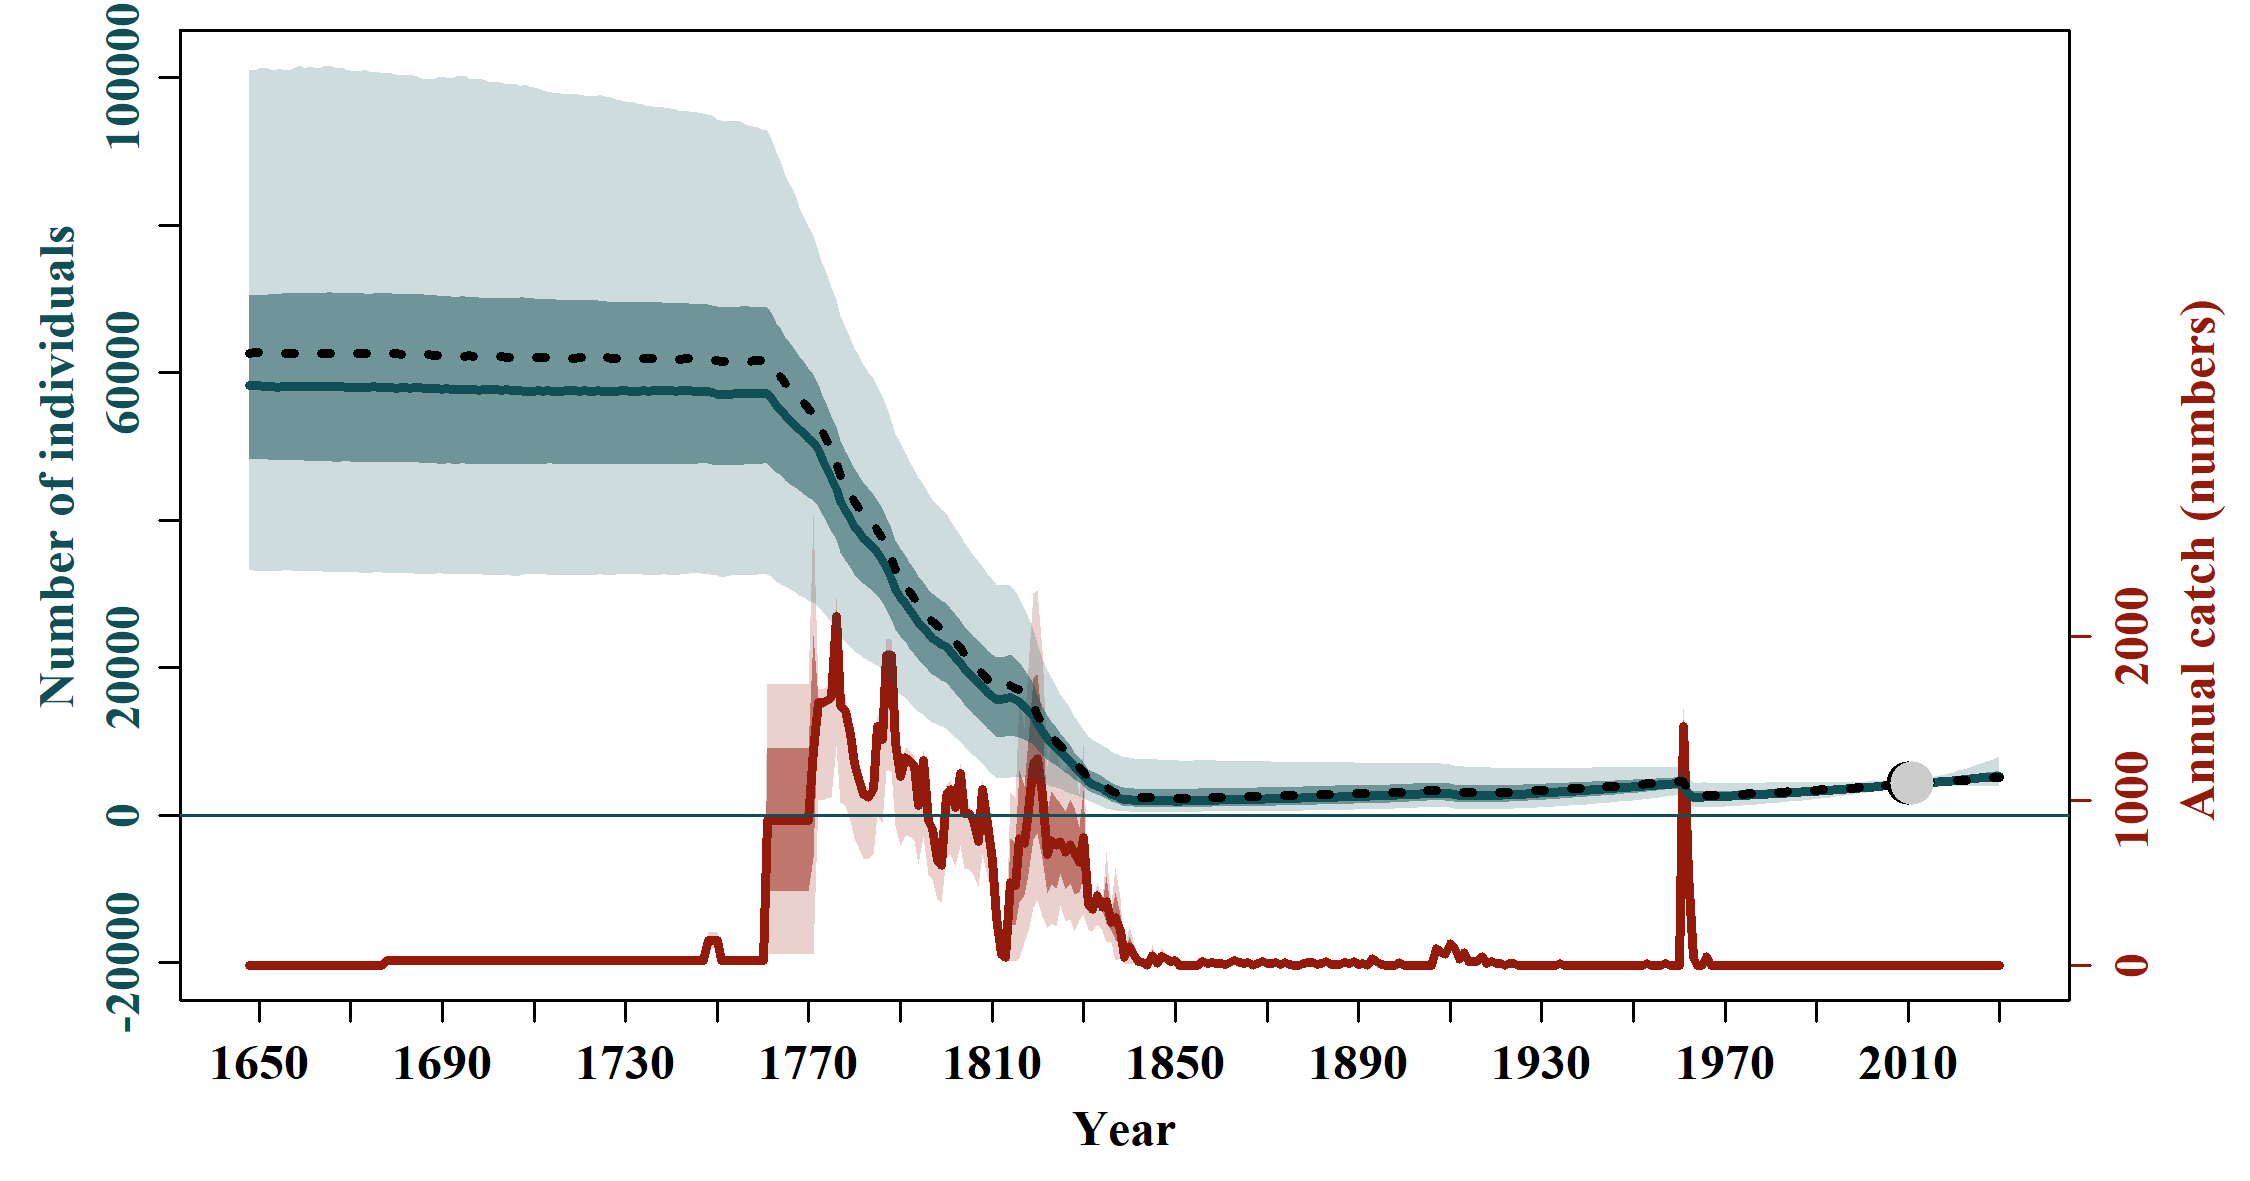
\includegraphics{Model runs/Model_average/Model_average_trajectory_summary.png}
\caption{\textbf{Figure 1.} Model averaged population trajectories (blue
lines) and time series of estimated catches (red lines) of southern
right whale (SRW) Eubalaena australis. The solid blue line represents
the median estimated model-averaged trajectory of the population
abundance (N\_y), while the shaded areas correspond to the 50\% and 95\%
credible intervals. The dashed line represents the median estimated base
case trajectory of the abundance. The solid red line represents the
average number of whaling catches as estimated by the catch parameter
(π), while the red shaded areas correspond to the 50\% and 95\% credible
intervals. The grey and black dots represent the estimated and observed,
respectively, absolute abundance in 2010 (confidence and credible
intervals can be found in Figure 4).}
\end{figure}

\newpage

\begin{figure}
\centering
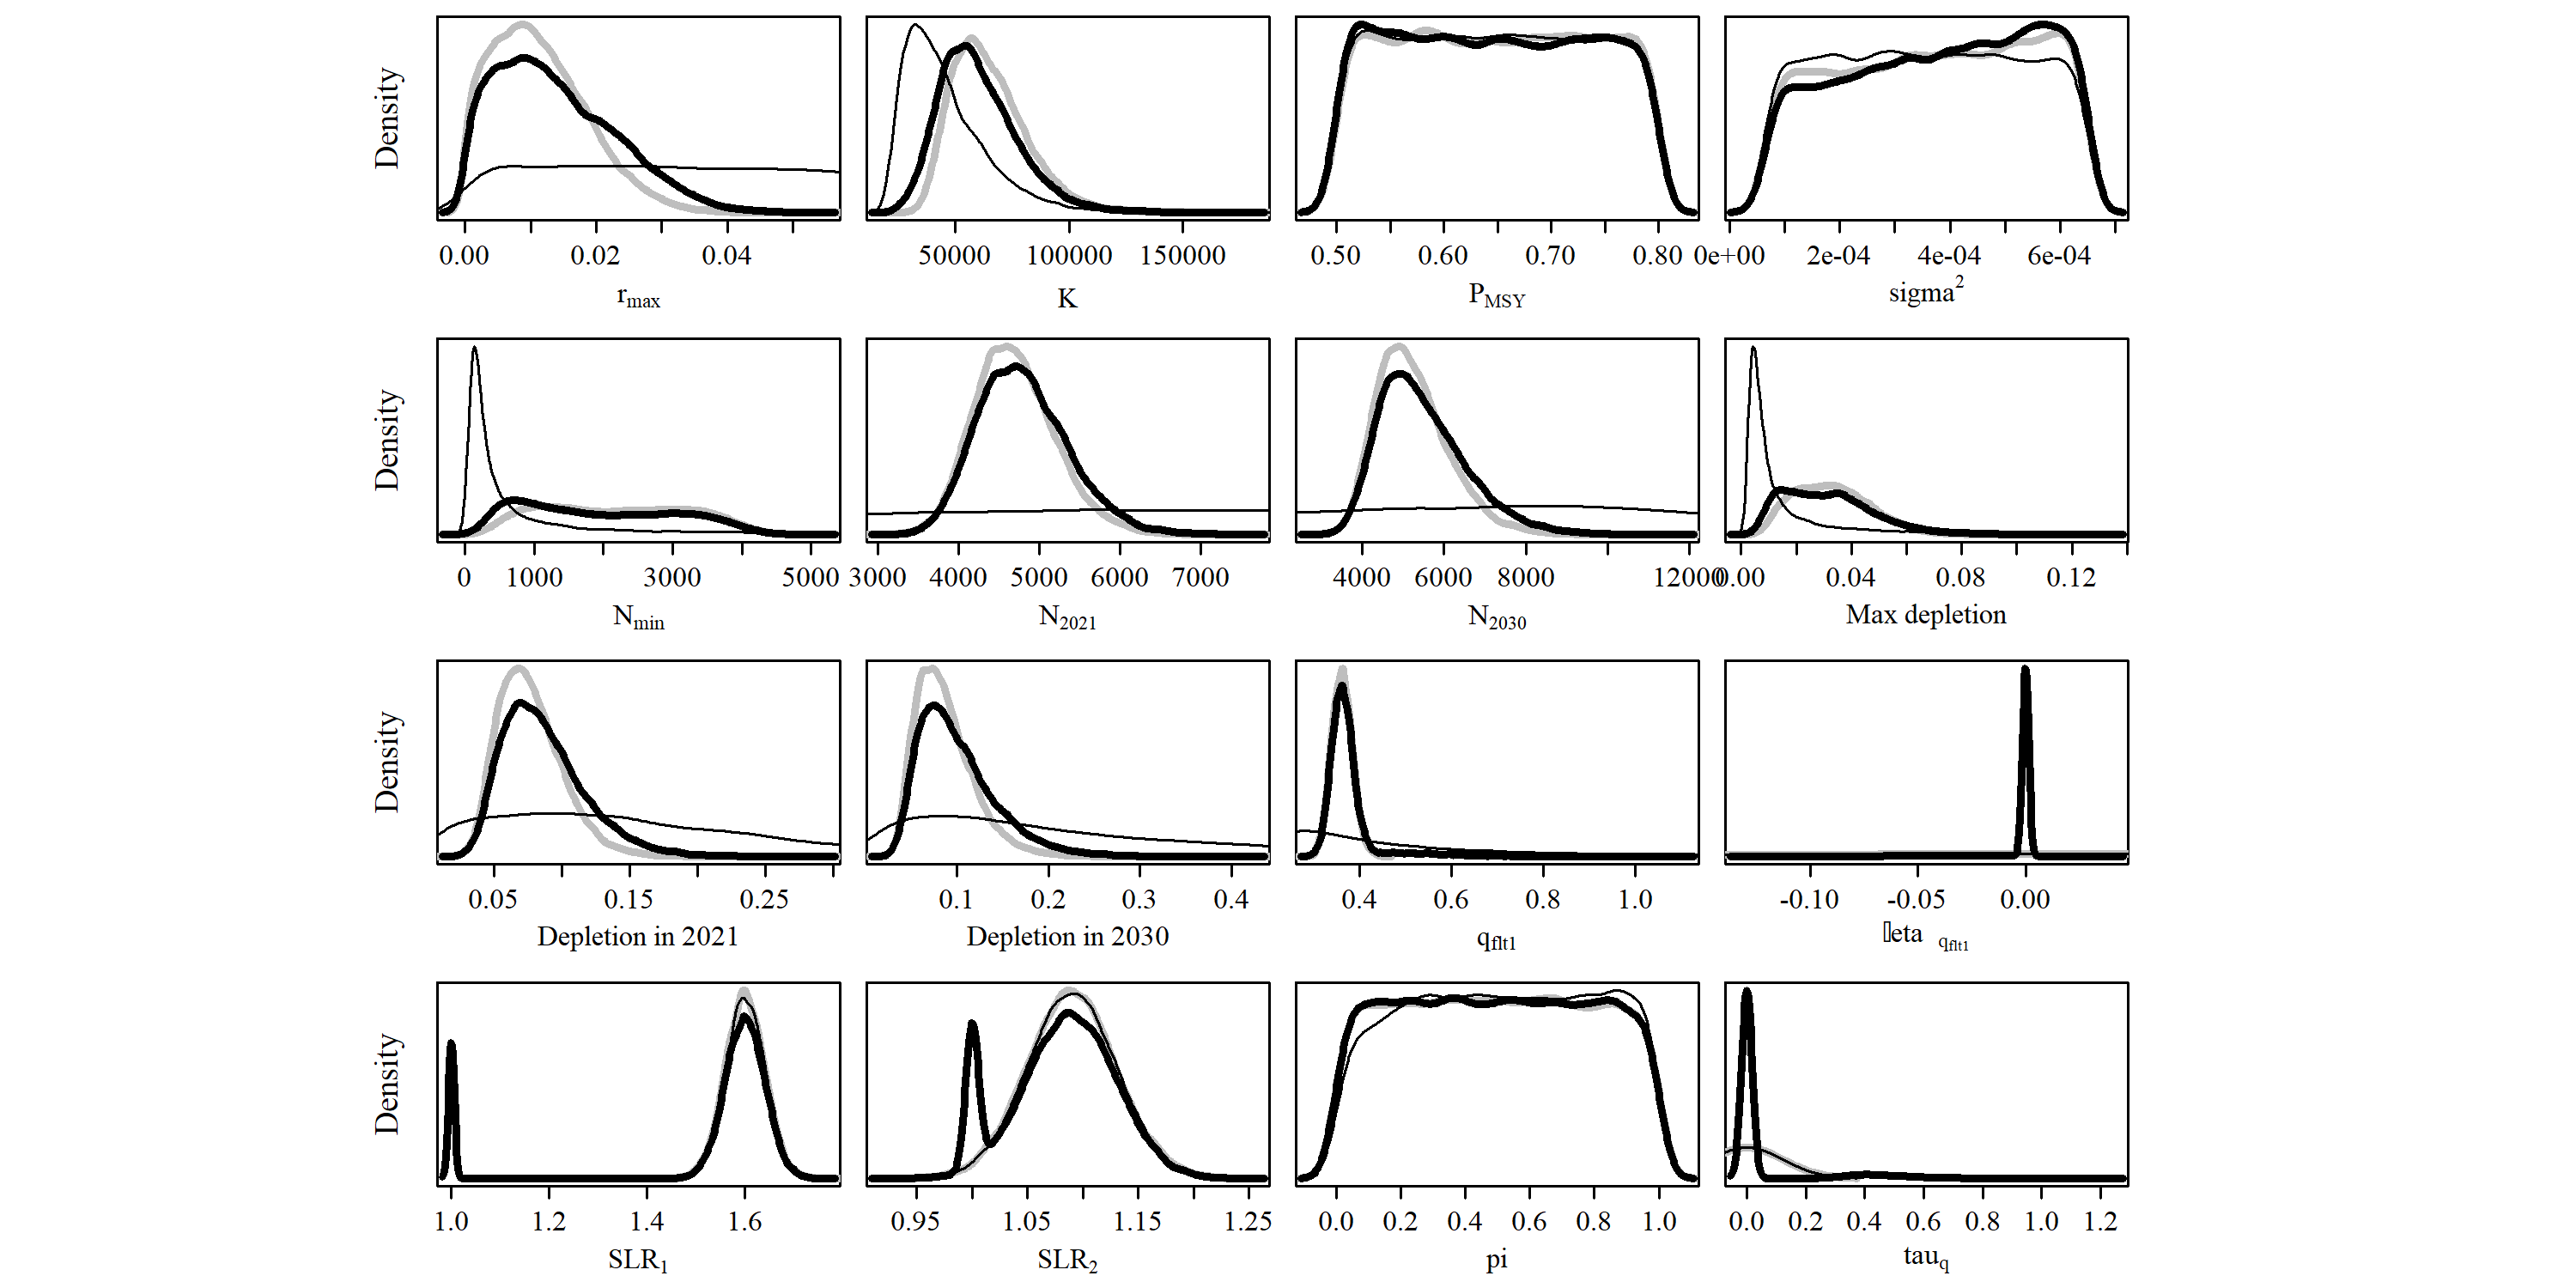
\includegraphics{Model runs/Model_average/Model_average_posterior_density.png}
\caption{\textbf{Figure 2.} Posterior probability distributions of the
key biological parameters for the 2023 Base Case (thick grey line) and
model-averaged (thick black line) assessment of southern right whale
(SRW) Eubalaena australis. Post-model pre-data probability distributions
of the key biological parameters for the Base Case are presented in the
thin grey line.}
\end{figure}

\newpage

\begin{figure}
\centering
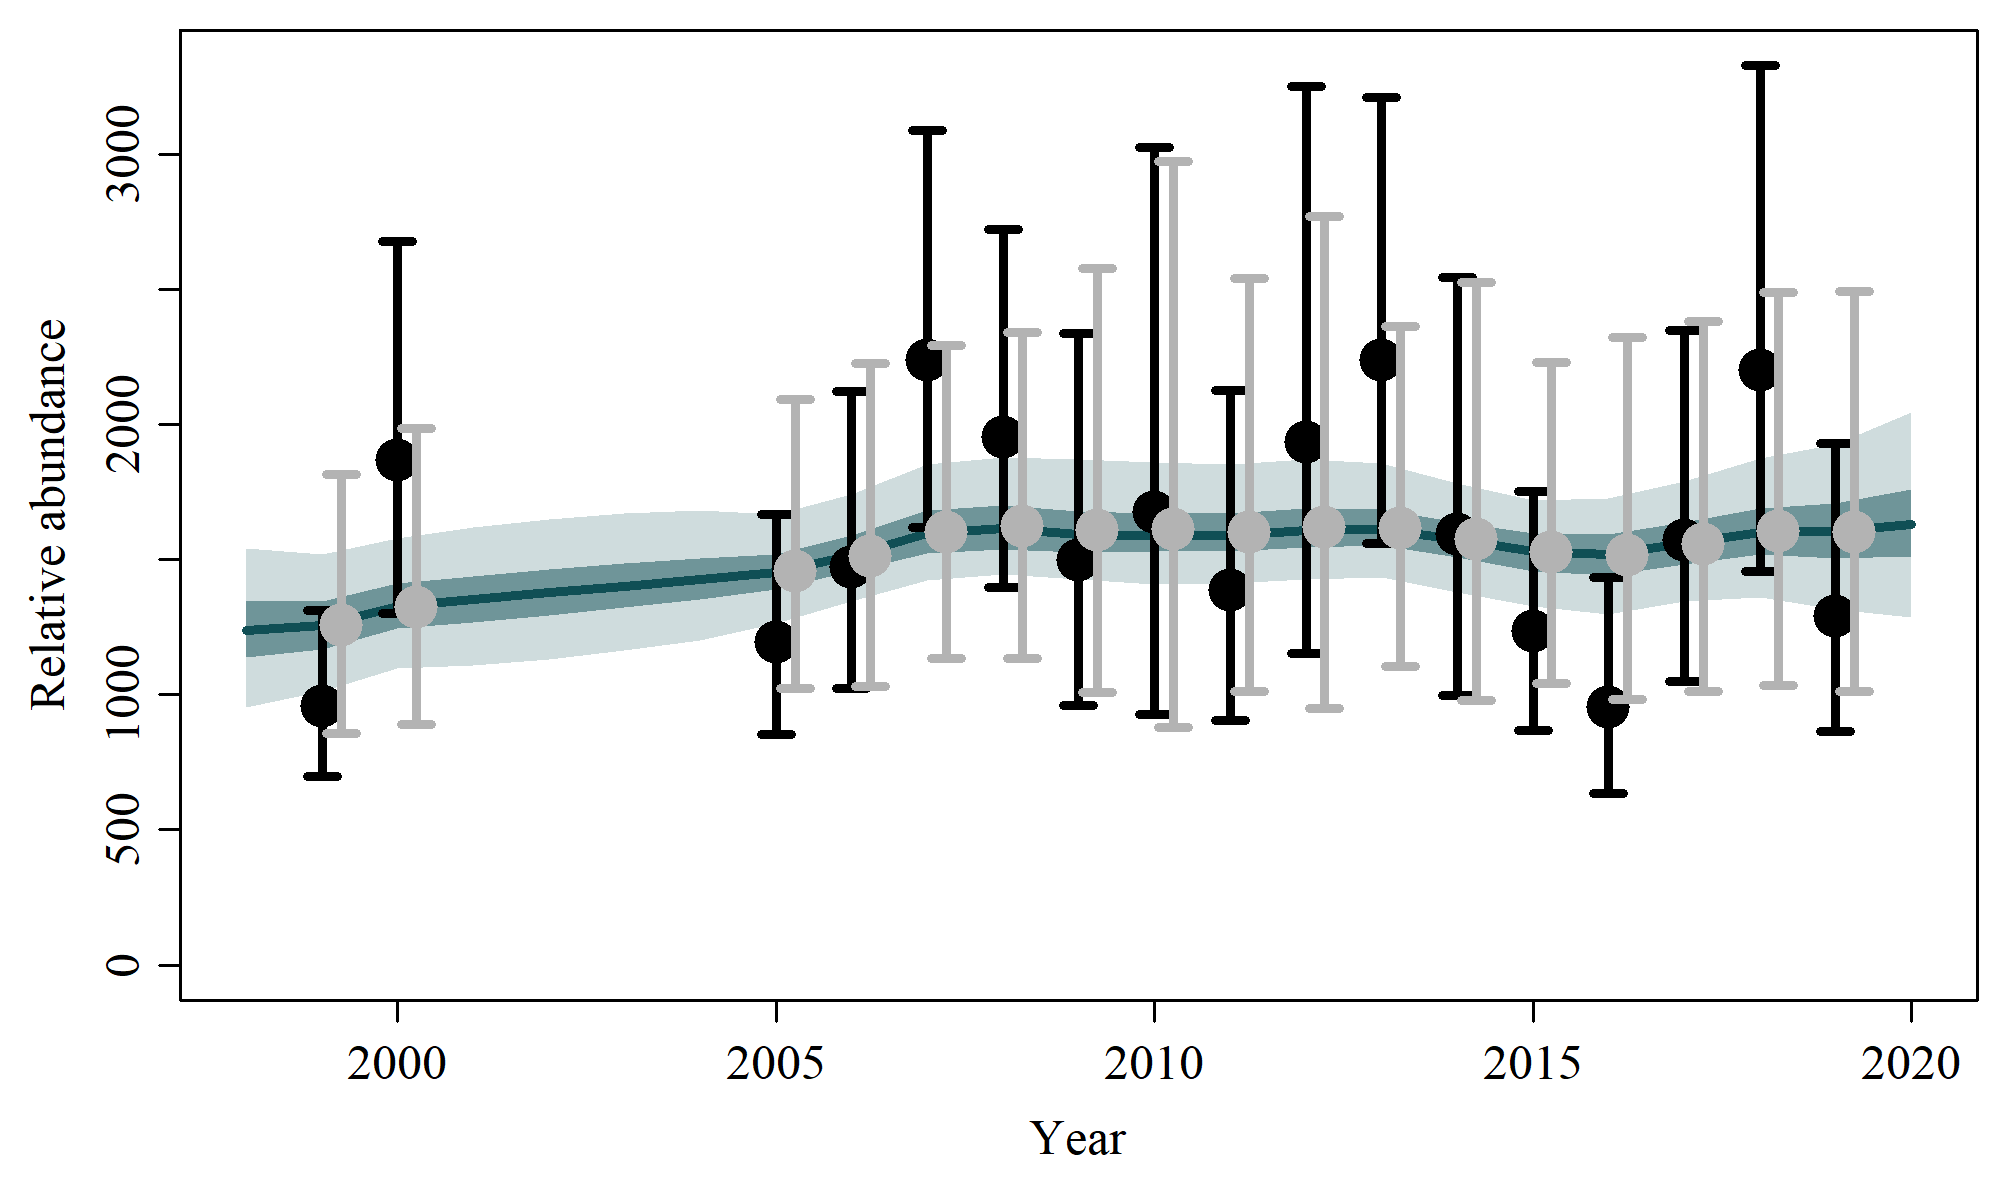
\includegraphics{Model runs/Model_average/Model_average_IOA_fit.png}
\caption{\textbf{Figure 3.} Trend of the observed (black dots) and
estimated (grey dots) accumulated numbers of the southern right whale
Eubalaena australis and associated 95\% confidence interval (black bars)
and 95\% posterior predictive intervals (grey bars). The solid blue line
represents the median estimated model-averaged trajectory of the
population abundance (N\_y) multiplied by posterior catchability (q),
while the shaded areas correspond to the 50\% and 95\% credible
intervals.}
\end{figure}

\newpage

\begin{figure}
\centering
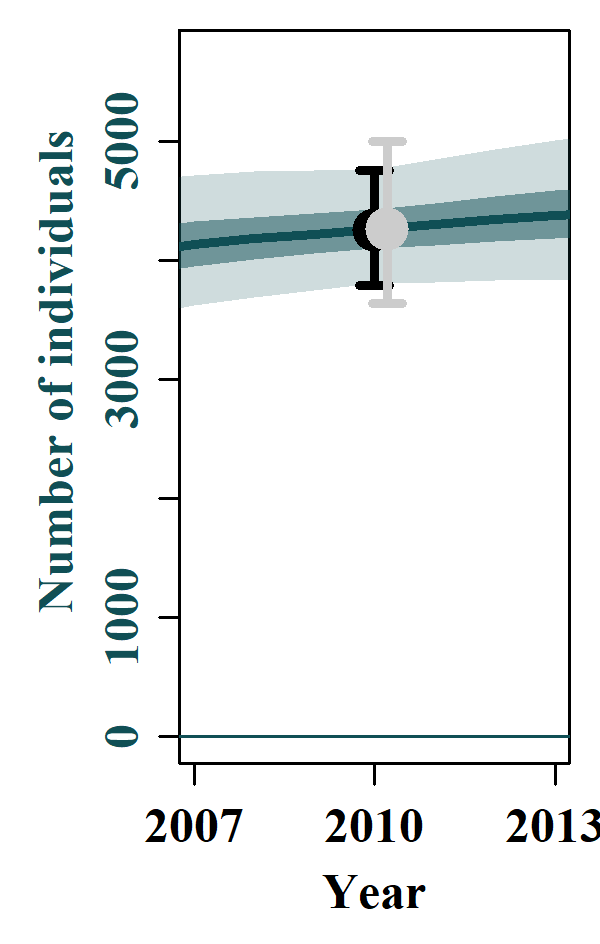
\includegraphics{Model runs/Model_average/Model_average_abs_abundance_fit.png}
\caption{\textbf{Figure 4.} Fits of the observed (black dots) and
estimated (grey dots) absolute abundance of southern right whale
Eubalaena australis and associated 95\% confidence interval (black bars)
and 95\% posterior predictive intervals (grey bars). The blue line is
the median abundance trajectory and the shaded areas correspond to the
50\% and 95\% credible intervals.}
\end{figure}

\end{document}
